%%%% 補助スライド
\appendix
\backupbegin
%%%%%%%%%%%%%%%%%%%%%%%%%%%%%%%%%%%%%%%%%%%%%%%%%%%%%%%%%%%%%%%%%%%
\begin{frame}{}
  \begin{center}\Huge
    Appendix
  \end{center}
\end{frame}
%%%%%%%%%%%%%%%%%%%%%%%%%%%%%%%%%%%%%%%%%%%%%%%%%%%%%%%%%%%%%%%%%%%
\begin{frame}\frametitle{実験結果: 解けた問題数}

  \begin{exampleblock}{}
    \centering
    \renewcommand{\arraystretch}{1.2}
    \scalebox{0.9}{\begin{tabular}{l|rr|rr} 
  & \multicolumn{2}{c|}{基本ソルバー} & \multicolumn{2}{c}{改良ソルバー} \\
  & \code{changed} & \code{unchanged} & \code{changed} & \code{unchanged} \\ \hline
  解けた問題数(到達可能) & 11 & 11 & 11 & 11 \\
  解けた問題数(到達不能) & 10 & 10 & 56 & \alert{60} \\\hline
  平均 CPU 時間(秒) & 223.796 & 151.341 & 101.758 & \alert{59.095} \\
\end{tabular}}
  \end{exampleblock}

  \begin{itemize}
  \item 90問中71問について,到達可能性を判定できた.
    \begin{itemize}
    \item 到達可能11問,到達不能60問
    \end{itemize}
  \item recongo と\code{unchanged}符号化の組合せが,
    最も多くの問題を解いた.平均CPU時間も最も短い.
%  \item 到達可能であることが判定できた問題のうち,最長のステップ長は17であった.
  \item 到達不能なインスタンスについて,インクリメンタル解法を用いた改
    良ソルバーの優位性が確認できた.
  \end{itemize}
\end{frame}
%%%%%%%%%%%%%%%%%%%%%%%%%%%%%%%%%%%%%%%%%%%%%%%%%%%%%%%%%%%%%%%%% 
\begin{frame}
  \frametitle{有界組合せ遷移の基本アイデア (提案)}
  \begin{itemize}
  \item 基の組合せ問題の変数集合
    $\bm{x} = \{x_1,x_2,\ldots,x_n\}$
    に対して,ステップ$t\geq 0$での各変数の値を表す変数集合
    $\bm{x}^{t} = \{x_1^t,x_2^t,\ldots,x_n^t\}$を導入.
  \item スタート状態から$\ell$ステップ遷移した後の各変数の値
    $\bm{x}^{\ell}$が,ゴール状態を満足するかを判定するため,
    論理式$\varphi_{\ell}$を構成する.
  \end{itemize}
  \begin{block}{}\centering\vskip-1em
  \begin{align*}
  \varphi_{\ell} &= S(\bm{x}^0)  & S: \textrm{スタート制約を表す論理式} \\
  &\land \bigwedge_{t=0}^{\ell} C(\bm{x}^t) & C: \textrm{組合せ制約を表す論理式} \\
  &\land \bigwedge_{t=1}^{\ell} T(\bm{x}^{t-1},\bm{x}^{t}) & T: \textrm{遷移制約を表す論理式} \\
  &\land G(\bm{x}^\ell)  & G: \textrm{ゴール制約を表す論理式}
  \end{align*}
  \end{block}
  \begin{itemize}
  \item \bm{$\varphi_{\ell}$}が充足可能の場合,
    ステップ長$\ell$の到達可能な遷移系列が存在する
    ことを意味する.
  \end{itemize}
\end{frame}
%%%%%%%%%%%%%%%%%%%%%%%%%%%%%%%%%%%%%%%%%%%%%%%%%%%%%%%%%%%%%%%%%%%
\begin{frame}[shrink]{有界組合せ遷移アルゴリズム}

  \begin{alertblock}{}\centering
  有界組合せ遷移のためのアルゴリズムを2種類考案した.
  \end{alertblock}
  
  \begin{center}
  \setlength{\unitlength}{1.0pt}
  \scriptsize\tiny
  \thicklines
  %    \thicklines
  \setlength{\unitlength}{1.28pt}
  \small
  \begin{picture}(280,57)(4,-10)
    \put(  0, 20){\dashbox(50,24){\shortstack{根付き全域森\\問題}}}
    \put( 60, 20){\framebox(50,24){変換器}}
    \put(120, 20){\dashbox(50,24){\shortstack{ASPファクト}}}
    \put(120,-10){\alert{\bf\dashbox(50,24){\scriptsize{\shortstack{ASP符号化\\(論理プログラム)}}}}}
    \put(180, 20){\framebox(50,24){ASPシステム}}
    \put(240, 20){\dashbox(50,24){\shortstack{根付き全域森\\問題の解}}}
    \put( 50, 32){\vector(1,0){10}}
    \put(110, 32){\vector(1,0){10}}
    \put(170, 32){\vector(1,0){10}}
    \put(230, 32){\vector(1,0){10}}
    \put(170, +2){\line(1,0){4}}
    \put(174, +2){\line(0,1){30}}
  \end{picture}  

  \begin{picture}(280,57)(4,-10)
    \put(  0, 20){\dashbox(50,24){\shortstack{組合せ遷移問題\\のインスタンス}}}
    \put( 60, 20){\framebox(50,24){変換器}}
    \put(120, 20){\dashbox(50,24){\shortstack{ASPファクト}}}
    \put(120,-10){\dashbox(50,24){\shortstack{論理プログラム\\(ASP符号化)}}}
    \put(180,-10){\framebox(50,54){}}
    \put(185, 27){\framebox(40,12){ASP システム}}
    \put(185, -5){\alert{\bf\framebox(40,18){\shortstack{有界組合せ遷移\\アルゴリズム}}}}
    \put(240, 20){\dashbox(50,24){\shortstack{組合せ遷移問題\\の解}}}
    \put( 50, 32){\vector(1,0){10}}
    \put(110, 32){\vector(1,0){10}}
    \put(170, 32){\vector(1,0){10}}
    \put(230, 32){\vector(1,0){10}}
    \put(170, +2){\line(1,0){4}}
    \put(174, +2){\line(0,1){30}}
    \put(195, 13){\vector(0,1){14}}
    \put(215, 27){\vector(0,-1){14}}
    \put(188, 50){提案ソルバー}
  \end{picture}  
  \end{center}
    
  \begin{enumerate}
  \item \structure{基本アルゴリズム}
    \begin{itemize}
    \item ステップ長$\ell$を増加させながら,
      $\varphi_{\ell}$を繰り返し構成し解く.
    \item 長所: 実装が単純である.
    \item 短所: 学習節が再利用できない.
    \item 短所: ASPシステムを毎回起動するオーバーヘッドが大きい.
    \end{itemize}
  \item \structure{インクリメンタルASP解法を用いた改良アルゴリズム}
    \begin{itemize}
    \item $S(\bm{x}^{0})$, $C(\bm{x}^{t})$,
      $T(\bm{x}^{t-1},\bm{x}^{t})$, $G(\bm{x}^{t})$
      を動的に追加・削除しながら,$\varphi_{\ell}$をインクリメンタルに構成し解く.
    \item 長所: 学習節の再利用が可能.ASPシステムの起動は1回のみ.
    \item 短所: 現状では,デバックしにくい.
    \end{itemize}
  \end{enumerate}
  \end{frame}

%%%%%%%%%%%%%%%%%%%%%%%%%%%%%%%%%%%%%%%%%%%%%%%%%%%%%%%%%%%%%%%%% 
%\begin{frame}%[shrink]
%  \frametitle{有界組合せ遷移 (提案)} 
%  \begin{alertblock}{有界組合せ遷移}\centering
%    組合せ遷移問題に対して,制限された長さ (すなわち,有界)の
%    遷移系列
%    \[
%    \varphi_{\ell} = S(\bm{x}^0)  
%    \land \bigwedge_{t=0}^{\ell} C(\bm{x}^t) 
%    \land \bigwedge_{t=1}^{\ell} T(\bm{x}^{t-1},\bm{x}^{t}) 
%    \land G(\bm{x}^\ell)  
%    \]
%    を論理プログラムとして表現し,
%    ASP システムを用いて実行することにより,到達可能性の検査を行う手法
%  \end{alertblock}
%  \begin{itemize}
%  \item $\varphi_{\ell}$が\structure{充足可能}の場合,
%    ステップ長$\ell$の\structure{到達可能}な遷移系列が存在.
%  \item \structure{充足不能}の場合,ステップ長$\ell$では\structure{到達不能}.
%    この場合,$\ell$を増加させた論理プログラムを再構成し,
%    繰り返し ASP システムを実行.
%  \item この手法は,到達不能の証明は行わない不完全な手続きである.
%    \begin{itemize}
%      \item ただし,検査すべき遷移系列のステップ長に上限~\footnotemark[2]
%        が存在する場合には,完全な手続きとなる.
%    \end{itemize}
%  \end{itemize}
%  \footnotetext[2]{例えば,任意の2つの実行可能解の最短経路のうちの最大長(問題の直径)}
%\end{frame}
%%%%%%%%%%%%%%%%%%%%%%%%%%%%%%%%%%%%%%%%%%%%%%%%%%%%%%%%%%%%%%%%%%%
\begin{frame}
  \frametitle{到達可能の判定に要したCPU時間}

  \begin{exampleblock}{}
    \centering
    \scalebox{0.75}{\begin{tabular}{lr|rr|rr}
  \multicolumn{2}{r|}{} & \multicolumn{2}{c|}{基本ソルバー} & \multicolumn{2}{c}{改良ソルバー} \\
  問題名 & ステップ長 & \code{changed} & \code{unchanged} & \code{changed} & \code{unchanged} \\ \hline
  \code{1-FullIns_3_col4_1} & 11 & 1.374 & 1.071 & 1.291 & 0.756 \\
  \code{myciel3_col4_1} & 11 & 0.179 & 0.148 & 0.065 & 0.065 \\
  \code{myciel3_col4_3} & 11 & 0.206 & 0.164 & 0.082 & 0.080 \\
  \code{myciel3_col4_4} & 13 & 0.486 & 0.445 & 0.303 & 0.583 \\
  \code{myciel3_col4_7} & 8 & 0.090 & 0.072 & 0.042 & 0.036 \\
  \code{myciel3_col4_8} & 9 & 0.119 & 0.094 & 0.048 & 0.044 \\
  \code{myciel4_col5_2} & 16 & 42.482 & 48.721 & 20.308 & 134.056 \\
  \code{myciel4_col5_3} & 14 & 17.098 & 21.211 & 5.286 & 80.848 \\
  \code{myciel4_col5_4} & 7 & 0.256 & 0.193 & 0.086 & 0.072 \\
  \code{myciel4_col5_6} & 10 & 1.525 & 1.391 & 1.052 & 1.558 \\
  \code{myciel4_col5_10} & 17 & 212.682 & 73.646 & 29.999 & 200.068 \\
\end{tabular}}
  \end{exampleblock}
  \begin{itemize}
    \item ステップ長については,最大で長さ17の問題が解けた.
    % \item 全体の結果とは異なる傾向が見られた.
    %   \begin{itemize}
    %     \item 十分な長さの遷移系列が最短の解となるようなベンチマークが必要である.
    %   \end{itemize}
  \end{itemize}
\end{frame}
%%%%%%%%%%%%%%%%%%%%%%%%%%%%%%%%%%%%%%%%%%%%%%%%%%%%%%%%%%%%%%%%%%% 
\begin{frame}
  \frametitle{基となるグラフごとの解けた問題数}
  
  \begin{exampleblock}{}
    \centering
    \scalebox{0.8}{\begin{tabular}{l|rrr|rrr}
  グラフ名 & 平均次数 & 色数$k$ & 実行可能解の総数 & 到達可能 & 到達不能 & 判定不能 \\ \hline
  1-FullIns\_3 & 6.67 & 4 & 50,693,280 & 1 & 0 & \structure{9} \\ 
  le450\_5a & 25.40 & 5 & 3,840 & 0 & 10 & 0 \\ 
  le450\_5c & 43.57 & 5 & 120 & 0 & 10 & 0 \\ 
  le450\_5d & 43.36 & 5 & 960 & 0 & 10 & 0 \\ 
  myciel3 & 3.64 & 4 & 12,480 & 5 & 0 & \structure{5} \\ 
  myciel4 & 6.17 & 5 & 2,845,658,400 & 5 & 0 & \structure{5} \\ 
  queen5\_5 & 12.80 & 5 & 240 & 0 & 10 & 0 \\  
  queen6\_6 & 16.11 & 7 & 100,800 & 0 & 10 & 0 \\ 
  queen7\_7 & 19.43 & 7 & 20,160 & 0 & 10 & 0 \\
\end{tabular}}
  \end{exampleblock}
  \begin{itemize}
    \item $\textrm{平均次数} = (\textrm{辺数}*2) / (\textrm{頂点数})$
    \item 色数$k$は彩色数に等しい.
    \item 難しい問題の特徴としては,基となる問題の実行可能解の総数が多いことや,
      平均次数と色数$k$の差が少ないことなどが考えられる.
      \begin{itemize}
        \item $k \ge \Delta(G) + 2$ならば到達可能である.
        \item $\Delta(G)$はグラフ$G$の最大次数である.
      \end{itemize}
  \end{itemize}
\end{frame}
%%%%%%%%%%%%%%%%%%%%%%%%%%%%%%%%%%%%%%%%%%%%%%%%%%%%%%%%%%%%%%%%%%%
\begin{frame}\frametitle{独立集合問題を基とする遷移問題}

  \begin{exampleblock}{サイズ$k=3$の独立集合問題}
    \begin{itemize}
      \item 制約を満たすように$k$個のトークンを配置する問題.
    \end{itemize}
    \centering
    \begin{tabular}[t]{ccc}
      \scalebox{0.55}{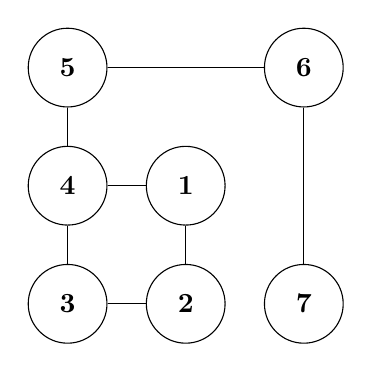
\begin{tikzpicture}[x=1.5cm, y=1.5cm]
  % 設定
  \tikzset{node/.style={circle,draw=black,minimum size=1cm}}
 
  % 補助線
  % \draw [help lines,blue] (0,0) grid (20,6);
 
  % node %
  \node[node] at (0,0) (node1) {\textbf{1}};
  \node[node] at (0,-1) (node2) {\textbf{2}};
  \node[node] at (-1,-1) (node3) {\textbf{3}};
  \node[node] at (-1,0) (node4) {\textbf{4}};
  \node[node] at (-1,1) (node5) {\textbf{5}};
  \node[node] at (1,1) (node6) {\textbf{6}};
  \node[node] at (1,-1) (node7) {\textbf{7}};
 
  \foreach \u / \v in {node1/node2, node1/node4, node2/node3, node3/node4, node4/node5,
    node5/node6, node6/node7}
  \draw (\u) -- (\v);
\end{tikzpicture}

}
      &
      \rz{$\Rightarrow$}
      &
      \scalebox{0.55}{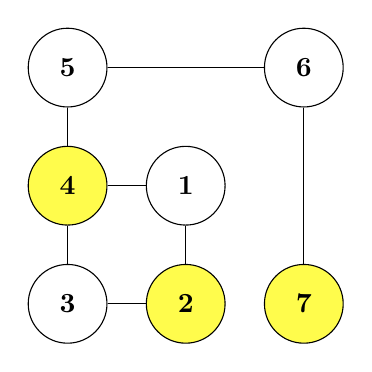
\begin{tikzpicture}[x=1.5cm, y=1.5cm]
  % 設定
  \tikzset{node/.style={circle,draw=black,minimum size=1cm}}
 
  % 色
  \definecolor{yellow}{RGB}{255,251,0}
 
  % 補助線
  % \draw [help lines,blue] (0,0) grid (20,6);
 
  % node %
  \node[node] at (0,0) (node1) {\textbf{1}};
  \node[node, fill=yellow!70] at (0,-1) (node2) {\textbf{2}};
  \node[node] at (-1,-1) (node3) {\textbf{3}};
  \node[node, fill=yellow!70] at (-1,0) (node4) {\textbf{4}};
  \node[node] at (-1,1) (node5) {\textbf{5}};
  \node[node] at (1,1) (node6) {\textbf{6}};
  \node[node, fill=yellow!70] at (1,-1) (node7) {\textbf{7}};
 
  \foreach \u / \v in {node1/node2, node1/node4, node2/node3, node3/node4, node4/node5,
    node5/node6, node6/node7}
  \draw (\u) -- (\v);
\end{tikzpicture}
}
    \end{tabular}
  \end{exampleblock}
  %
  \begin{block}{独立集合遷移問題: モデル Token Jumping (TJ)}
    \begin{itemize}
      \item \structure{\bf 入力}:
        サイズ$k$の独立集合問題と,スタート状態とゴール状態
        を表す2つの実行可能解
      \item \structure{遷移制約}: 1回の遷移でただ1つのトークンが移動する
      \item \structure{目的}:
        スタート状態からゴール状態への到達可能性を判定
      \end{itemize}
  \end{block}
  \begin{itemize}
    \item 遷移制約をより厳しくしたモデルである Token Sliding (TS) も存在.
  \end{itemize}
\end{frame}
%%%%%%%%%%%%%%%%%%%%%%%%%%%%%%%%%%%%%%%%%%%%%%%%%%%%%%%%%%%%%%%%%
\begin{frame}%[shrink]
  \frametitle{$k=3$の独立集合遷移問題の例\footnote{伊藤健洋,第1回 CoRe.Seminar スライドより}}
  \begin{center}
  \tabcolsep = 3mm
  \renewcommand{\arraystretch}{1.2}
  \begin{tabular}[t]{ccc}
    スタート状態($t=0$) && \uncover<2>{$t=1$} \\
    \scalebox{0.5}{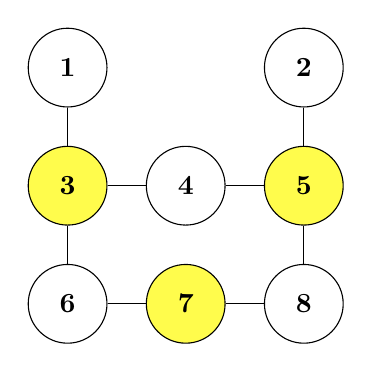
\begin{tikzpicture}[x=1.5cm, y=1.5cm]
  % 設定
  \tikzset{node/.style={circle,draw=black,minimum size=1cm}}
 
  % 色
  \definecolor{yellow}{RGB}{255,251,0}
 
  % 補助線
  % \draw [help lines,blue] (0,0) grid (20,6);
 
  % node %
  \node[node] at (-1,1) (node1) {\textbf{1}};
  \node[node] at (1,1) (node2) {\textbf{2}};
  \node[node, fill=yellow!70] at (-1,0) (node3) {\textbf{3}};
  \node[node] at (0,0) (node4) {\textbf{4}};
  \node[node, fill=yellow!70] at (1,0) (node5) {\textbf{5}};
  \node[node] at (-1,-1) (node6) {\textbf{6}};
  \node[node, fill=yellow!70] at (0,-1) (node7) {\textbf{7}};
  \node[node] at (1,-1) (node8) {\textbf{8}};
 
  \foreach \u / \v in {node1/node3, node2/node5, node3/node4, node3/node6, node4/node5,
    node5/node8, node6/node7, node7/node8}
  \draw (\u) -- (\v);
\end{tikzpicture}
} &
    \uncover<2>{\rz{\Large$\Rightarrow$}} &
    \uncover<2>{\scalebox{0.5}{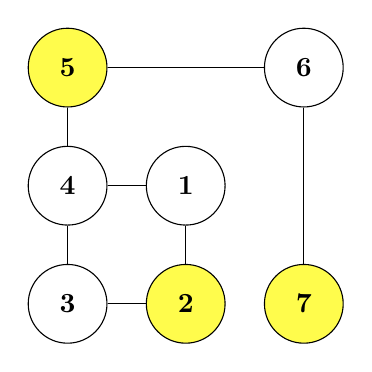
\begin{tikzpicture}[x=1.5cm, y=1.5cm]
  % 設定
  \tikzset{node/.style={circle,draw=black,minimum size=1cm}}
 
  % 色
  \definecolor{yellow}{RGB}{255,251,0}
 
  % 補助線
  % \draw [help lines,blue] (0,0) grid (20,6);
 
  % node %
  \node[node] at (0,0) (node1) {\textbf{1}};
  \node[node, fill=yellow!70] at (0,-1) (node2) {\textbf{2}};
  \node[node] at (-1,-1) (node3) {\textbf{3}};
  \node[node] at (-1,0) (node4) {\textbf{4}};
  \node[node, fill=yellow!70] at (-1,1) (node5) {\textbf{5}};
  \node[node] at (1,1) (node6) {\textbf{6}};
  \node[node, fill=yellow!70] at (1,-1) (node7) {\textbf{7}};
 
  \foreach \u / \v in {node1/node2, node1/node4, node2/node3, node3/node4, node4/node5,
    node5/node6, node6/node7}
  \draw (\u) -- (\v);
\end{tikzpicture}
}}\\
    && \uncover<2>{\Large $\Downarrow$} \\
    \scalebox{0.5}{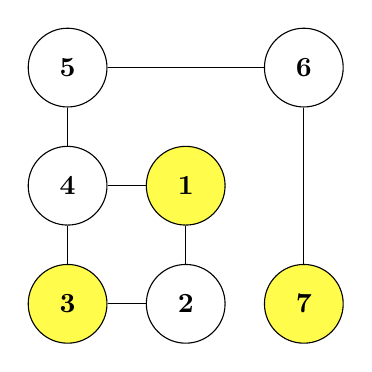
\begin{tikzpicture}[x=1.5cm, y=1.5cm]
  % 設定
  \tikzset{node/.style={circle,draw=black,minimum size=1cm}}
 
  % 色
  \definecolor{yellow}{RGB}{255,251,0}
 
  % 補助線
  % \draw [help lines,blue] (0,0) grid (20,6);
 
  % node %
  \node[node, fill=yellow!70] at (0,0) (node1) {\textbf{1}};
  \node[node] at (0,-1) (node2) {\textbf{2}};
  \node[node, fill=yellow!70] at (-1,-1) (node3) {\textbf{3}};
  \node[node] at (-1,0) (node4) {\textbf{4}};
  \node[node] at (-1,1) (node5) {\textbf{5}};
  \node[node] at (1,1) (node6) {\textbf{6}};
  \node[node, fill=yellow!70] at (1,-1) (node7) {\textbf{7}};
 
  \foreach \u / \v in {node1/node2, node1/node4, node2/node3, node3/node4, node4/node5,
    node5/node6, node6/node7}
  \draw (\u) -- (\v);
\end{tikzpicture}
} &
    \uncover<2>{\rz{\Large$\Leftarrow$}} &
    \uncover<2>{\scalebox{0.5}{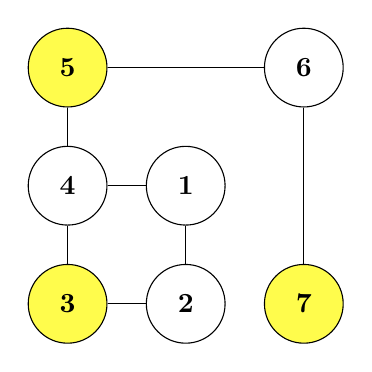
\begin{tikzpicture}[x=1.5cm, y=1.5cm]
  % 設定
  \tikzset{node/.style={circle,draw=black,minimum size=1cm}}
 
  % 色
  \definecolor{yellow}{RGB}{255,251,0}
 
  % 補助線
  % \draw [help lines,blue] (0,0) grid (20,6);
 
  % node %
  \node[node] at (0,0) (node1) {\textbf{1}};
  \node[node] at (0,-1) (node2) {\textbf{2}};
  \node[node, fill=yellow!70] at (-1,-1) (node3) {\textbf{3}};
  \node[node] at (-1,0) (node4) {\textbf{4}};
  \node[node, fill=yellow!70] at (-1,1) (node5) {\textbf{5}};
  \node[node] at (1,1) (node6) {\textbf{6}};
  \node[node, fill=yellow!70] at (1,-1) (node7) {\textbf{7}};
 
  \foreach \u / \v in {node1/node2, node1/node4, node2/node3, node3/node4, node4/node5,
    node5/node6, node6/node7}
  \draw (\u) -- (\v);
\end{tikzpicture}
}}\\
    ゴール状態\uncover<2>{($t=3$)} && \uncover<2>{$t=2$}
  \end{tabular}
  \end{center}

  \uncover<2>{
  \begin{itemize}
  \item スタート状態からゴール状態へ3ステップで到達可能である.
  \item 各ステップ$t$において,独立集合問題の制約を満たす.
  \item 1回の遷移において,移動するトークンはただ1つのみである.
  \end{itemize}
  }
\end{frame}
%%%%%%%%%%%%%%%%%%%%%%%%%%%%%%%%%%%%%%%%%%%%%%%%%%%%%%%%%%%%%%%%%%%
\backupend

%%% Local Variables:
%%% mode: japanese-latex
%%% TeX-master: "slides"
%%% End:
